\documentclass{beamer}
\usepackage[utf8]{inputenc}
  
\usetheme{Madrid}
\usecolortheme{default}
\usepackage{amsmath,amssymb,amsfonts,amsthm}
\usepackage{txfonts}
\usepackage{tkz-euclide}
\usepackage{listings}
\usepackage{adjustbox}
\usepackage{array}
\usepackage{tabularx}
\usepackage{gvv}
\usepackage{lmodern}
\usepackage{circuitikz}
\usepackage{tikz}
\usepackage{graphicx}
\usepackage[T1]{fontenc}
\UseRawInputEncoding

\setbeamertemplate{page number in head/foot}[totalframenumber]

\usepackage{tcolorbox}
\tcbuselibrary{minted,breakable,xparse,skins}



\definecolor{bg}{gray}{0.95}
\DeclareTCBListing{mintedbox}{O{}m!O{}}{%
  breakable=true,
  listing engine=minted,
  listing only,
  minted language=#2,
  minted style=default,
  minted options={%
    linenos,
    gobble=0,
    breaklines=true,
    breakafter=,,
    fontsize=\small,
    numbersep=8pt,
    #1},
  boxsep=0pt,
  left skip=0pt,
  right skip=0pt,
  left=25pt,
  right=0pt,
  top=3pt,
  bottom=3pt,
  arc=5pt,
  leftrule=0pt,
  rightrule=0pt,
  bottomrule=2pt,
  toprule=2pt,
  colback=bg,
  colframe=orange!70,
  enhanced,
  overlay={%
    \begin{tcbclipinterior}
    \fill[orange!20!white] (frame.south west) rectangle ([xshift=20pt]frame.north west);
    \end{tcbclipinterior}},
  #3,
}
\lstset{
    language=C,
    basicstyle=\ttfamily\small,
    keywordstyle=\color{blue},
    stringstyle=\color{orange},
    commentstyle=\color{green!60!black},
    numbers=left,
    numberstyle=\tiny\color{gray},
    breaklines=true,
    showstringspaces=false,
}



\title 
{MatGeo Assignment 4.12.12}

\author
{AI25BTECH11007}
\begin{document}

\frame{\titlepage}
\begin{frame}{Question}
For what values of a and b the intercepts cut off on the coordinate axes by the line ax+by+8 = 0 are equal in length but opposite in signs to those cut off by the line 2x-3y = 0 on the axes.
\end{frame}

\begin{frame}{Solution}
    \[
\text{Line :} ax+by+8=0 
\quad\Longleftrightarrow\quad 
\myvec{a & b} \myvec{x \\ y} + 8 = 0
\]
         
\[
\text{Intercept vector: }
\myvec{-\tfrac{8}{a} \\[2mm] -\tfrac{8}{b}}
\]

\[
\text{For } 2x-3y=0 \;\;\Longleftrightarrow\;\; 
\frac{x}{3}+\frac{y}{-2}=0,
\quad
\text{intercept vector: }
\myvec{3 \\ -2}
\]

\[
\text{Condition: }\;
\myvec{-\tfrac{8}{a} \\[2mm] -\tfrac{8}{b}}
=
-\myvec{3 \\ -2}
\]

\[
\Rightarrow\quad 
-\frac{8}{a} = -3, 
\quad 
-\frac{8}{b} = 2
\]

\[
\Rightarrow\quad 
a = \tfrac{8}{3}, 
\quad 
b = -4
\]

\end{frame}

\begin{frame}{Plot}
    \begin{figure}
        \centering
        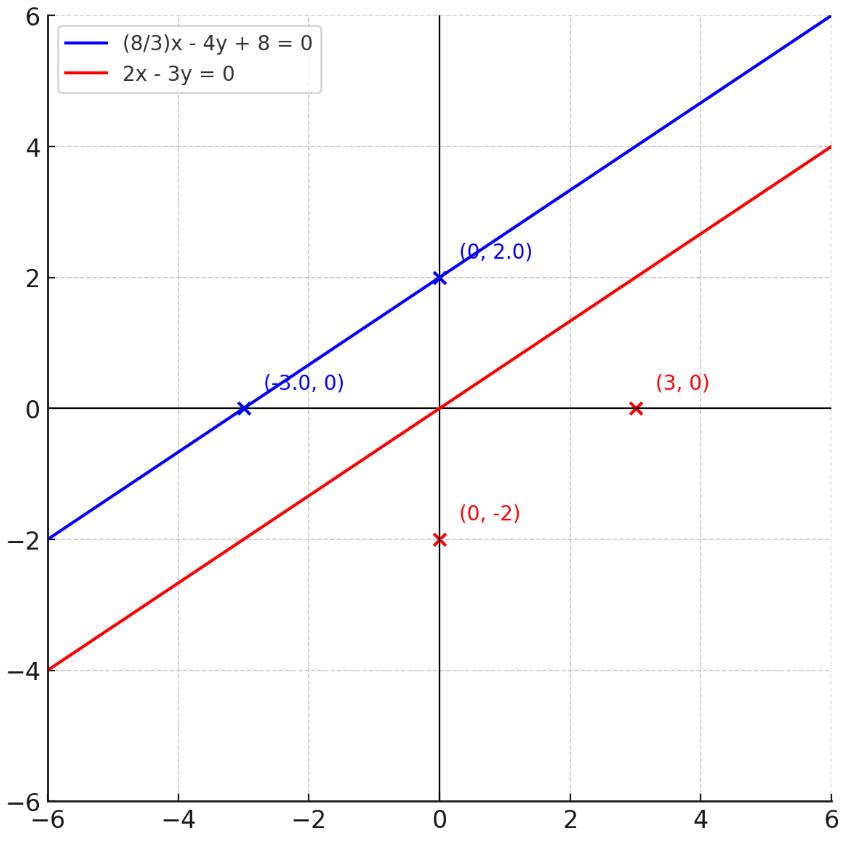
\includegraphics[width=0.60\linewidth]{figs/image.png}
        \caption{Plot}
        \label{fig:placeholder}
    \end{figure}
\end{frame}

\begin{frame}[fragile]{C code}
    \begin{lstlisting}
#include <stdio.h>
int main() {
    // Line 1: (8/3)x - 4y + 8 = 0
    float a = 8.0/3.0;
    float b = -4;
    // Intercepts of line 1
    float x1 = -8 / a;   // x-intercept
    float y1 = -8 / b;   // y-intercept
    // Line 2: 2x - 3y = 0
    // Intercepts of line 2
    float x2 = 3;
    float y2 = -2;
    printf("Line 1: (8/3)x - 4y + 8 = 0\n");
    printf("Intercepts: (%.1f, 0) and (0, %.1f)\n\n", x1, y1);
    printf("Line 2: 2x - 3y = 0\n");
    printf("Intercepts: (%.1f, 0) and (0, %.1f)\n", x2, y2);
    return 0;
}
    \end{lstlisting}
\end{frame}

\begin{frame}[fragile]{Python code}
    \begin{lstlisting}
        import matplotlib.pyplot as plt
import numpy as np
# Define the lines
x = np.linspace(-10, 10, 400)
# Line 1: (8/3)x - 4y + 8 = 0 -> y = (2/3)x + 2
y1 = (2/3)*x + 2
# Line 2: 2x - 3y = 0 -> y = (2/3)x
y2 = (2/3)*x
# Axes
fig, ax = plt.subplots(figsize=(6,6))
ax.axhline(0, color='black', linewidth=0.8)
ax.axvline(0, color='black', linewidth=0.8)
\end{lstlisting}
\end{frame}

\begin{frame}[fragile]{Python code}
\begin{lstlisting}
# Plot the lines
ax.plot(x, y1, 'r', label=r'$\tfrac{8}{3}x - 4y + 8 = 0$')
ax.plot(x, y2, 'b', label=r'$2x - 3y = 0$')

# Mark intercepts for line 1
x_int1 = -8/(8/3)  # = -3
y_int1 = -8/(-4)   # = 2
ax.scatter([x_int1, 0], [0, y_int1], color='red')
ax.text(x_int1, 0.5, f"(-3,0)", color="red", fontsize=9)
ax.text(0.3, y_int1, f"(0,2)", color="red", fontsize=9)

# Mark intercepts for line 2
x_int2 = 3
y_int2 = -2
ax.scatter([x_int2, 0], [0, y_int2], color='blue')
ax.text(x_int2, -0.7, f"(3,0)", color="blue", fontsize=9)
ax.text(0.3, y_int2, f"(0,-2)", color="blue", fontsize=9)
\end{lstlisting}
\end{frame}

\begin{frame}[fragile]{Python code}
\begin{lstlisting}
# Limits and grid
ax.set_xlim(-6, 6)
ax.set_ylim(-6, 6)
ax.grid(True, linestyle="--", alpha=0.6)
ax.legend()
plt.show()

    \end{lstlisting}
\end{frame}

\end{document}